% Figure from MATH 591 notes, section 72 (Lecture 27). After the board sketch (Lecture 27): canonical form near a regular point.
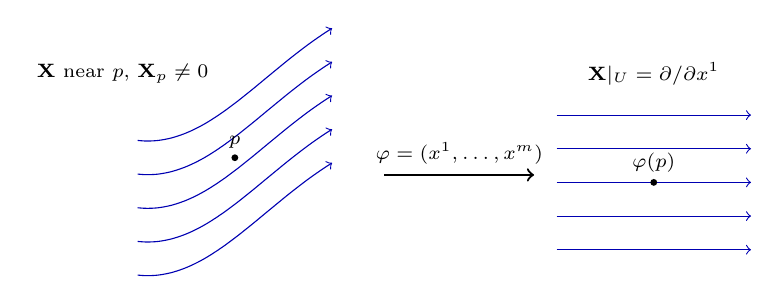
\begin{tikzpicture}[scale=0.95]
\draw[blue!70!black, ->] plot[smooth] coordinates {(-1.400,-1.239) (-1.310,-1.246) (-1.221,-1.246) (-1.131,-1.240) (-1.041,-1.226) (-0.952,-1.207) (-0.862,-1.180) (-0.772,-1.148) (-0.683,-1.110) (-0.593,-1.066) (-0.503,-1.017) (-0.414,-0.963) (-0.324,-0.904) (-0.234,-0.842) (-0.145,-0.776) (-0.055,-0.708) (0.034,-0.637) (0.124,-0.565) (0.214,-0.491) (0.303,-0.417) (0.393,-0.343) (0.483,-0.269) (0.572,-0.196) (0.662,-0.124) (0.752,-0.054) (0.841,0.014) (0.931,0.080) (1.021,0.143) (1.110,0.203) (1.200,0.261)};
\draw[blue!70!black, ->] plot[smooth] coordinates {(-1.400,-0.789) (-1.310,-0.796) (-1.221,-0.796) (-1.131,-0.790) (-1.041,-0.776) (-0.952,-0.757) (-0.862,-0.730) (-0.772,-0.698) (-0.683,-0.660) (-0.593,-0.616) (-0.503,-0.567) (-0.414,-0.513) (-0.324,-0.454) (-0.234,-0.392) (-0.145,-0.326) (-0.055,-0.258) (0.034,-0.187) (0.124,-0.115) (0.214,-0.041) (0.303,0.033) (0.393,0.107) (0.483,0.181) (0.572,0.254) (0.662,0.326) (0.752,0.396) (0.841,0.464) (0.931,0.530) (1.021,0.593) (1.110,0.653) (1.200,0.711)};
\draw[blue!70!black, ->] plot[smooth] coordinates {(-1.400,-0.339) (-1.310,-0.346) (-1.221,-0.346) (-1.131,-0.340) (-1.041,-0.326) (-0.952,-0.307) (-0.862,-0.280) (-0.772,-0.248) (-0.683,-0.210) (-0.593,-0.166) (-0.503,-0.117) (-0.414,-0.063) (-0.324,-0.004) (-0.234,0.058) (-0.145,0.124) (-0.055,0.192) (0.034,0.263) (0.124,0.335) (0.214,0.409) (0.303,0.483) (0.393,0.557) (0.483,0.631) (0.572,0.704) (0.662,0.776) (0.752,0.846) (0.841,0.914) (0.931,0.980) (1.021,1.043) (1.110,1.103) (1.200,1.161)};
\draw[blue!70!black, ->] plot[smooth] coordinates {(-1.400,0.111) (-1.310,0.104) (-1.221,0.104) (-1.131,0.110) (-1.041,0.124) (-0.952,0.143) (-0.862,0.170) (-0.772,0.202) (-0.683,0.240) (-0.593,0.284) (-0.503,0.333) (-0.414,0.387) (-0.324,0.446) (-0.234,0.508) (-0.145,0.574) (-0.055,0.642) (0.034,0.713) (0.124,0.785) (0.214,0.859) (0.303,0.933) (0.393,1.007) (0.483,1.081) (0.572,1.154) (0.662,1.226) (0.752,1.296) (0.841,1.364) (0.931,1.430) (1.021,1.493) (1.110,1.553) (1.200,1.611)};
\draw[blue!70!black, ->] plot[smooth] coordinates {(-1.400,0.561) (-1.310,0.554) (-1.221,0.554) (-1.131,0.560) (-1.041,0.574) (-0.952,0.593) (-0.862,0.620) (-0.772,0.652) (-0.683,0.690) (-0.593,0.734) (-0.503,0.783) (-0.414,0.837) (-0.324,0.896) (-0.234,0.958) (-0.145,1.024) (-0.055,1.092) (0.034,1.163) (0.124,1.235) (0.214,1.309) (0.303,1.383) (0.393,1.457) (0.483,1.531) (0.572,1.604) (0.662,1.676) (0.752,1.746) (0.841,1.814) (0.931,1.880) (1.021,1.943) (1.110,2.003) (1.200,2.061)};
\fill (-0.1,0.33) circle (1.3pt) node[above, font=\scriptsize] {$p$};
\node[font=\scriptsize] at (-1.6,1.45) {$\mathbf{X}$ near $p$, $\mathbf{X}_p \neq 0$};
\draw[->, thick] (1.9,0.1) -- node[above, font=\scriptsize] {$\varphi = (x^1, \ldots, x^m)$} (3.9,0.1);
\draw[blue!70!black, ->] (4.2,-0.9) -- (6.8,-0.9);
\draw[blue!70!black, ->] (4.2,-0.45) -- (6.8,-0.45);
\draw[blue!70!black, ->] (4.2,0.0) -- (6.8,0.0);
\draw[blue!70!black, ->] (4.2,0.45) -- (6.8,0.45);
\draw[blue!70!black, ->] (4.2,0.9) -- (6.8,0.9);
\fill (5.5,0.0) circle (1.3pt) node[above, font=\scriptsize] {$\varphi(p)$};
\node[font=\scriptsize] at (5.5,1.45) {$\mathbf{X}|_U = \partial/\partial x^1$};
\end{tikzpicture}
